% Options for packages loaded elsewhere
\PassOptionsToPackage{unicode}{hyperref}
\PassOptionsToPackage{hyphens}{url}
\PassOptionsToPackage{dvipsnames,svgnames,x11names}{xcolor}
%
\documentclass[
  letterpaper,
  DIV=11,
  numbers=noendperiod]{scrartcl}

\usepackage{amsmath,amssymb}
\usepackage{iftex}
\ifPDFTeX
  \usepackage[T1]{fontenc}
  \usepackage[utf8]{inputenc}
  \usepackage{textcomp} % provide euro and other symbols
\else % if luatex or xetex
  \usepackage{unicode-math}
  \defaultfontfeatures{Scale=MatchLowercase}
  \defaultfontfeatures[\rmfamily]{Ligatures=TeX,Scale=1}
\fi
\usepackage{lmodern}
\ifPDFTeX\else  
    % xetex/luatex font selection
\fi
% Use upquote if available, for straight quotes in verbatim environments
\IfFileExists{upquote.sty}{\usepackage{upquote}}{}
\IfFileExists{microtype.sty}{% use microtype if available
  \usepackage[]{microtype}
  \UseMicrotypeSet[protrusion]{basicmath} % disable protrusion for tt fonts
}{}
\makeatletter
\@ifundefined{KOMAClassName}{% if non-KOMA class
  \IfFileExists{parskip.sty}{%
    \usepackage{parskip}
  }{% else
    \setlength{\parindent}{0pt}
    \setlength{\parskip}{6pt plus 2pt minus 1pt}}
}{% if KOMA class
  \KOMAoptions{parskip=half}}
\makeatother
\usepackage{xcolor}
\setlength{\emergencystretch}{3em} % prevent overfull lines
\setcounter{secnumdepth}{-\maxdimen} % remove section numbering
% Make \paragraph and \subparagraph free-standing
\ifx\paragraph\undefined\else
  \let\oldparagraph\paragraph
  \renewcommand{\paragraph}[1]{\oldparagraph{#1}\mbox{}}
\fi
\ifx\subparagraph\undefined\else
  \let\oldsubparagraph\subparagraph
  \renewcommand{\subparagraph}[1]{\oldsubparagraph{#1}\mbox{}}
\fi

\usepackage{color}
\usepackage{fancyvrb}
\newcommand{\VerbBar}{|}
\newcommand{\VERB}{\Verb[commandchars=\\\{\}]}
\DefineVerbatimEnvironment{Highlighting}{Verbatim}{commandchars=\\\{\}}
% Add ',fontsize=\small' for more characters per line
\usepackage{framed}
\definecolor{shadecolor}{RGB}{241,243,245}
\newenvironment{Shaded}{\begin{snugshade}}{\end{snugshade}}
\newcommand{\AlertTok}[1]{\textcolor[rgb]{0.68,0.00,0.00}{#1}}
\newcommand{\AnnotationTok}[1]{\textcolor[rgb]{0.37,0.37,0.37}{#1}}
\newcommand{\AttributeTok}[1]{\textcolor[rgb]{0.40,0.45,0.13}{#1}}
\newcommand{\BaseNTok}[1]{\textcolor[rgb]{0.68,0.00,0.00}{#1}}
\newcommand{\BuiltInTok}[1]{\textcolor[rgb]{0.00,0.23,0.31}{#1}}
\newcommand{\CharTok}[1]{\textcolor[rgb]{0.13,0.47,0.30}{#1}}
\newcommand{\CommentTok}[1]{\textcolor[rgb]{0.37,0.37,0.37}{#1}}
\newcommand{\CommentVarTok}[1]{\textcolor[rgb]{0.37,0.37,0.37}{\textit{#1}}}
\newcommand{\ConstantTok}[1]{\textcolor[rgb]{0.56,0.35,0.01}{#1}}
\newcommand{\ControlFlowTok}[1]{\textcolor[rgb]{0.00,0.23,0.31}{#1}}
\newcommand{\DataTypeTok}[1]{\textcolor[rgb]{0.68,0.00,0.00}{#1}}
\newcommand{\DecValTok}[1]{\textcolor[rgb]{0.68,0.00,0.00}{#1}}
\newcommand{\DocumentationTok}[1]{\textcolor[rgb]{0.37,0.37,0.37}{\textit{#1}}}
\newcommand{\ErrorTok}[1]{\textcolor[rgb]{0.68,0.00,0.00}{#1}}
\newcommand{\ExtensionTok}[1]{\textcolor[rgb]{0.00,0.23,0.31}{#1}}
\newcommand{\FloatTok}[1]{\textcolor[rgb]{0.68,0.00,0.00}{#1}}
\newcommand{\FunctionTok}[1]{\textcolor[rgb]{0.28,0.35,0.67}{#1}}
\newcommand{\ImportTok}[1]{\textcolor[rgb]{0.00,0.46,0.62}{#1}}
\newcommand{\InformationTok}[1]{\textcolor[rgb]{0.37,0.37,0.37}{#1}}
\newcommand{\KeywordTok}[1]{\textcolor[rgb]{0.00,0.23,0.31}{#1}}
\newcommand{\NormalTok}[1]{\textcolor[rgb]{0.00,0.23,0.31}{#1}}
\newcommand{\OperatorTok}[1]{\textcolor[rgb]{0.37,0.37,0.37}{#1}}
\newcommand{\OtherTok}[1]{\textcolor[rgb]{0.00,0.23,0.31}{#1}}
\newcommand{\PreprocessorTok}[1]{\textcolor[rgb]{0.68,0.00,0.00}{#1}}
\newcommand{\RegionMarkerTok}[1]{\textcolor[rgb]{0.00,0.23,0.31}{#1}}
\newcommand{\SpecialCharTok}[1]{\textcolor[rgb]{0.37,0.37,0.37}{#1}}
\newcommand{\SpecialStringTok}[1]{\textcolor[rgb]{0.13,0.47,0.30}{#1}}
\newcommand{\StringTok}[1]{\textcolor[rgb]{0.13,0.47,0.30}{#1}}
\newcommand{\VariableTok}[1]{\textcolor[rgb]{0.07,0.07,0.07}{#1}}
\newcommand{\VerbatimStringTok}[1]{\textcolor[rgb]{0.13,0.47,0.30}{#1}}
\newcommand{\WarningTok}[1]{\textcolor[rgb]{0.37,0.37,0.37}{\textit{#1}}}

\providecommand{\tightlist}{%
  \setlength{\itemsep}{0pt}\setlength{\parskip}{0pt}}\usepackage{longtable,booktabs,array}
\usepackage{calc} % for calculating minipage widths
% Correct order of tables after \paragraph or \subparagraph
\usepackage{etoolbox}
\makeatletter
\patchcmd\longtable{\par}{\if@noskipsec\mbox{}\fi\par}{}{}
\makeatother
% Allow footnotes in longtable head/foot
\IfFileExists{footnotehyper.sty}{\usepackage{footnotehyper}}{\usepackage{footnote}}
\makesavenoteenv{longtable}
\usepackage{graphicx}
\makeatletter
\def\maxwidth{\ifdim\Gin@nat@width>\linewidth\linewidth\else\Gin@nat@width\fi}
\def\maxheight{\ifdim\Gin@nat@height>\textheight\textheight\else\Gin@nat@height\fi}
\makeatother
% Scale images if necessary, so that they will not overflow the page
% margins by default, and it is still possible to overwrite the defaults
% using explicit options in \includegraphics[width, height, ...]{}
\setkeys{Gin}{width=\maxwidth,height=\maxheight,keepaspectratio}
% Set default figure placement to htbp
\makeatletter
\def\fps@figure{htbp}
\makeatother

\KOMAoption{captions}{tableheading}
\makeatletter
\@ifpackageloaded{caption}{}{\usepackage{caption}}
\AtBeginDocument{%
\ifdefined\contentsname
  \renewcommand*\contentsname{Table of contents}
\else
  \newcommand\contentsname{Table of contents}
\fi
\ifdefined\listfigurename
  \renewcommand*\listfigurename{List of Figures}
\else
  \newcommand\listfigurename{List of Figures}
\fi
\ifdefined\listtablename
  \renewcommand*\listtablename{List of Tables}
\else
  \newcommand\listtablename{List of Tables}
\fi
\ifdefined\figurename
  \renewcommand*\figurename{Figure}
\else
  \newcommand\figurename{Figure}
\fi
\ifdefined\tablename
  \renewcommand*\tablename{Table}
\else
  \newcommand\tablename{Table}
\fi
}
\@ifpackageloaded{float}{}{\usepackage{float}}
\floatstyle{ruled}
\@ifundefined{c@chapter}{\newfloat{codelisting}{h}{lop}}{\newfloat{codelisting}{h}{lop}[chapter]}
\floatname{codelisting}{Listing}
\newcommand*\listoflistings{\listof{codelisting}{List of Listings}}
\makeatother
\makeatletter
\makeatother
\makeatletter
\@ifpackageloaded{caption}{}{\usepackage{caption}}
\@ifpackageloaded{subcaption}{}{\usepackage{subcaption}}
\makeatother
\ifLuaTeX
  \usepackage{selnolig}  % disable illegal ligatures
\fi
\usepackage{bookmark}

\IfFileExists{xurl.sty}{\usepackage{xurl}}{} % add URL line breaks if available
\urlstyle{same} % disable monospaced font for URLs
\hypersetup{
  pdftitle={Regressão Linear no RStudio},
  pdfauthor={Saulo Morellato},
  colorlinks=true,
  linkcolor={blue},
  filecolor={Maroon},
  citecolor={Blue},
  urlcolor={Blue},
  pdfcreator={LaTeX via pandoc}}

\title{Regressão Linear no RStudio}
\author{Saulo Morellato}
\date{}

\begin{document}
\maketitle

\section{Introdução}\label{introduuxe7uxe3o}

\subsection{Objetivo Geral}\label{objetivo-geral}

Estabelecer uma função que descreva a relação entre uma variável
contínua \(Y\) (variável resposta) e uma ou mais variáveis de apoio
\(X_1, X_2,\dots, X_p\) (covariáveis) na forma
\[Y=f(X_1,X_2,\ldots,X_p)+\epsilon\] sendo \(\epsilon\) um erro
aleatório.

\subsection{Erro Aleatório}\label{erro-aleatuxf3rio}

Possíveis explicações para a presença do erro aleatório no modelo são:

\begin{itemize}
\item
  Caráter vago da teoria;
\item
  Falta de dados disponíveis;
\item
  Caráter aleatório da natureza;
\item
  Escolha equivocada para a forma funcional.
\end{itemize}

\section{Regressão Linear}\label{regressuxe3o-linear}

\subsection{Objetivo}\label{objetivo}

\begin{itemize}
\item
  Na Análise de Regressão Linear o objetivo é identificar uma equação
  linear que permita descrever o comportamento da variável resposta
  \(Y\) utilizando valores conhecidos das covariáveis
  \(X1,X2,\ldots,Xp\).
\item
  Ou seja, considera-se que a função \(f(\cdot)\) tenha uma forma
  linear.
\end{itemize}

\subsection{Regressão Linear Simples}\label{regressuxe3o-linear-simples}

Temos apenas uma covariável no modelo. Um exemplo seria tentar modelar o
quanto as despesas com propaganda inflenciam nas vendas de um
determinado produto.

\begin{itemize}
\item
  Variável resposta: \emph{vendas}
\item
  Covariável: \emph{gasto com propagandas}
\end{itemize}

\subsection{Regressão Linear
Múltipla}\label{regressuxe3o-linear-muxfaltipla}

Temos apenas duas ou mais covariáveis no modelo. Um exemplo seria tentar
modelar o quanto as características de um imóvel influenciam no preço de
venda do mesmo.

\begin{itemize}
\item
  Variável resposta: \emph{preço do imóvel}
\item
  Covariáveis: \emph{área, no de quartos, no de banheiros,
  idade,\ldots{}}
\end{itemize}

\section{Modelo Matemático}\label{modelo-matemuxe1tico}

\subsection{Descrição do Modelo}\label{descriuxe7uxe3o-do-modelo}

\begin{itemize}
\item
  A forma funcional é linear;
\item
  Considera-se apenas uma covariável;
\item
  Desse modo, temos \[Y=\beta_0+\beta_1X+\epsilon\]
\item
  \(\beta_0\) e \(\beta_1\) são valores desconhecidos (parâmetros) da
  reta que relaciona \(X\) e \(Y\);
\item
  \(\beta_0\) é chamado de intercepto; e
\item
  \(\beta_1\) é o coeficiente angular.
\end{itemize}

\subsection{Exemplo}\label{exemplo}

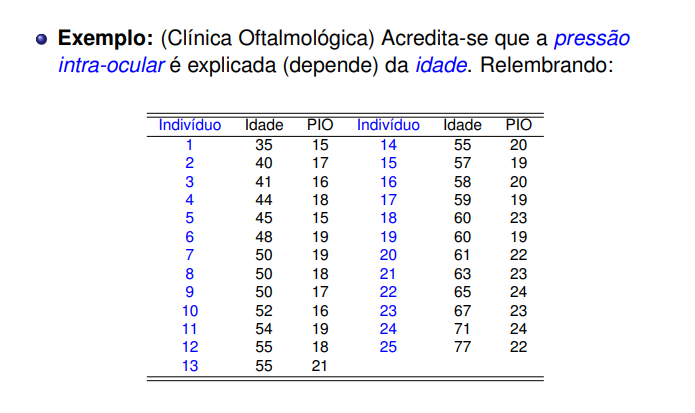
\includegraphics[width=0.8\textwidth,height=\textheight]{dados_pio.png}

\subsection{Exemplo (continuação)}\label{exemplo-continuauxe7uxe3o}

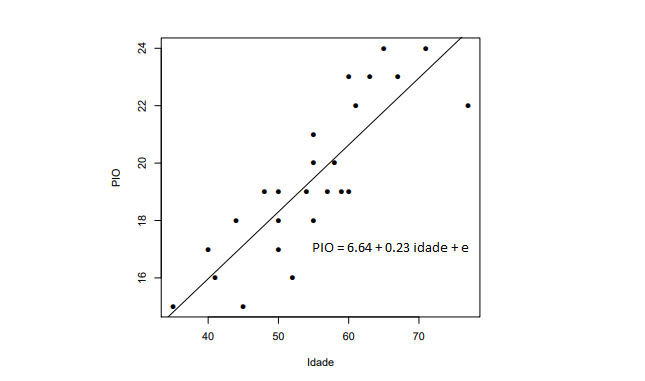
\includegraphics[width=0.8\textwidth,height=\textheight]{graf_pio.png}

\section{Aplicação em R}\label{aplicauxe7uxe3o-em-r}

\subsection{Carregando Pacotes}\label{carregando-pacotes}

\begin{itemize}
\item
  Para exemplificar a estimação de um modelo de Regressão Linear em R
  vamos utilizar conjunto de dados \texttt{dados\_imoveis.csv}.
\item
  Para isso primeiramente vamos carregar os pacotes necessários.
\end{itemize}

\begin{Shaded}
\begin{Highlighting}[]
\FunctionTok{library}\NormalTok{(tidyverse)  }\CommentTok{\# para organizar os dados}
\FunctionTok{library}\NormalTok{(gtsummary)  }\CommentTok{\# para organizar resultados em tabela}
\FunctionTok{library}\NormalTok{(mixlm)      }\CommentTok{\# para selecao de variaveis (stepwise)}
\end{Highlighting}
\end{Shaded}

\begin{Shaded}
\begin{Highlighting}[]
\NormalTok{code}\FunctionTok{.sourceCode}\NormalTok{ \{}
  \KeywordTok{font{-}size}\CharTok{:} \DecValTok{1.5}\DataTypeTok{em}\OperatorTok{;}
  \CommentTok{/* or try font{-}size: xx{-}large; */}
\NormalTok{\}}
\end{Highlighting}
\end{Shaded}

\subsection{Carregando e Manipulando
Dados}\label{carregando-e-manipulando-dados}

\begin{itemize}
\tightlist
\item
  Carregue o arquivo \texttt{dados\_imoveis.csv} utilizando o comando
  \texttt{read.csv()}.
\end{itemize}

\begin{Shaded}
\begin{Highlighting}[]
\NormalTok{dados}\OtherTok{\textless{}{-}} \FunctionTok{read.csv}\NormalTok{(}\StringTok{"dados\_imoveis.csv"}\NormalTok{, }\AttributeTok{header=}\ConstantTok{TRUE}\NormalTok{)}
\end{Highlighting}
\end{Shaded}

\begin{itemize}
\tightlist
\item
  Dê uma olhada superficial na estrutura dos dados usando o comando
  \texttt{glimpse()}.
\end{itemize}

\begin{Shaded}
\begin{Highlighting}[]
\FunctionTok{glimpse}\NormalTok{(dados)}
\end{Highlighting}
\end{Shaded}

\begin{itemize}
\tightlist
\item
  Transforme a variável \texttt{piscina} em fator, em seguida Verifique
  as estatísticas descritivas utlizando o comando \texttt{summary()}.
\end{itemize}

\begin{Shaded}
\begin{Highlighting}[]
\NormalTok{dados}\SpecialCharTok{$}\NormalTok{piscina}\OtherTok{\textless{}{-}} \FunctionTok{as.factor}\NormalTok{(dados}\SpecialCharTok{$}\NormalTok{piscina)}
\FunctionTok{summary}\NormalTok{(dados)}
\end{Highlighting}
\end{Shaded}

\begin{Shaded}
\begin{Highlighting}[]
\NormalTok{code}\FunctionTok{.sourceCode}\NormalTok{ \{}
  \KeywordTok{font{-}size}\CharTok{:} \DecValTok{1.5}\DataTypeTok{em}\OperatorTok{;}
  \CommentTok{/* or try font{-}size: xx{-}large; */}
\NormalTok{\}}
\end{Highlighting}
\end{Shaded}




\end{document}
